%%===========================================================%%
%%                                                           %%
%%                 WORKING POINT FOR CUTS                    %%
%%                                                           %%
%%===========================================================%%

\chapter{Working points optimization for cuts~\ref{enum:CutBbcLarge}, \ref{enum:CutTofClusters} and \ref{enum:CutMissingPt}}\label{appendix:workingPoint}

The described study has been done at an early stage of analysis with the fiducial region defined differently from that finally established, therefore it has not been contained in the main part of this note. However, we consider it helpful to justify the cut thresholds in three significant cuts given in the title of this appendix. For aforementioned reason final numbers (for nominal fiducial region) slightly differ from these presented in Fig.~\ref{fig:workingPoint}, but the general picture remains unchanged.

We define significance, efficiency, and purity of the three cuts: \ref{enum:CutBbcLarge}, \ref{enum:CutTofClusters} and \ref{enum:CutMissingPt}, according to equations shown below.\\[-15pt]%
\begin{tabulary}{\textwidth}{LLL}
\begin{equation}\label{eq:significance}\hspace*{-10pt}
	\text{Significance} = \frac{N_{\text{signal}}^{\text{cut}}}{\sqrt{N_{\text{signal}}^{\text{cut}} + N_{\text{bkgd}}^{\text{cut}}}},
\end{equation}~~~~~~~~~~~~~~~~~&
\begin{equation}\label{eq:efficiency}\hspace*{-10pt}
	\text{Efficiency} = \frac{N_{\text{signal}}^{\text{cut}}}{N_{\text{signal}}^{\text{no~cut}}},
\end{equation}~~~~~~~~~~~~~~&
\begin{equation}\label{eq:purity}\hspace*{-9pt}
	\text{Purity} = \frac{N_{\text{signal}}^{\text{cut}}}{N_{\text{signal}}^{\text{cut}}+N_{\text{bkgd}}^{\text{cut}}},
\end{equation}~~~~~~~~~~~~~~~
\end{tabulary}%
%--------------------------
\begin{figure}[b!]
\centering
\parbox{0.4725\textwidth}{
  \centering
  \begin{subfigure}[b]{\linewidth}
                \subcaptionbox{\label{fig:SignificanceVsEff}}{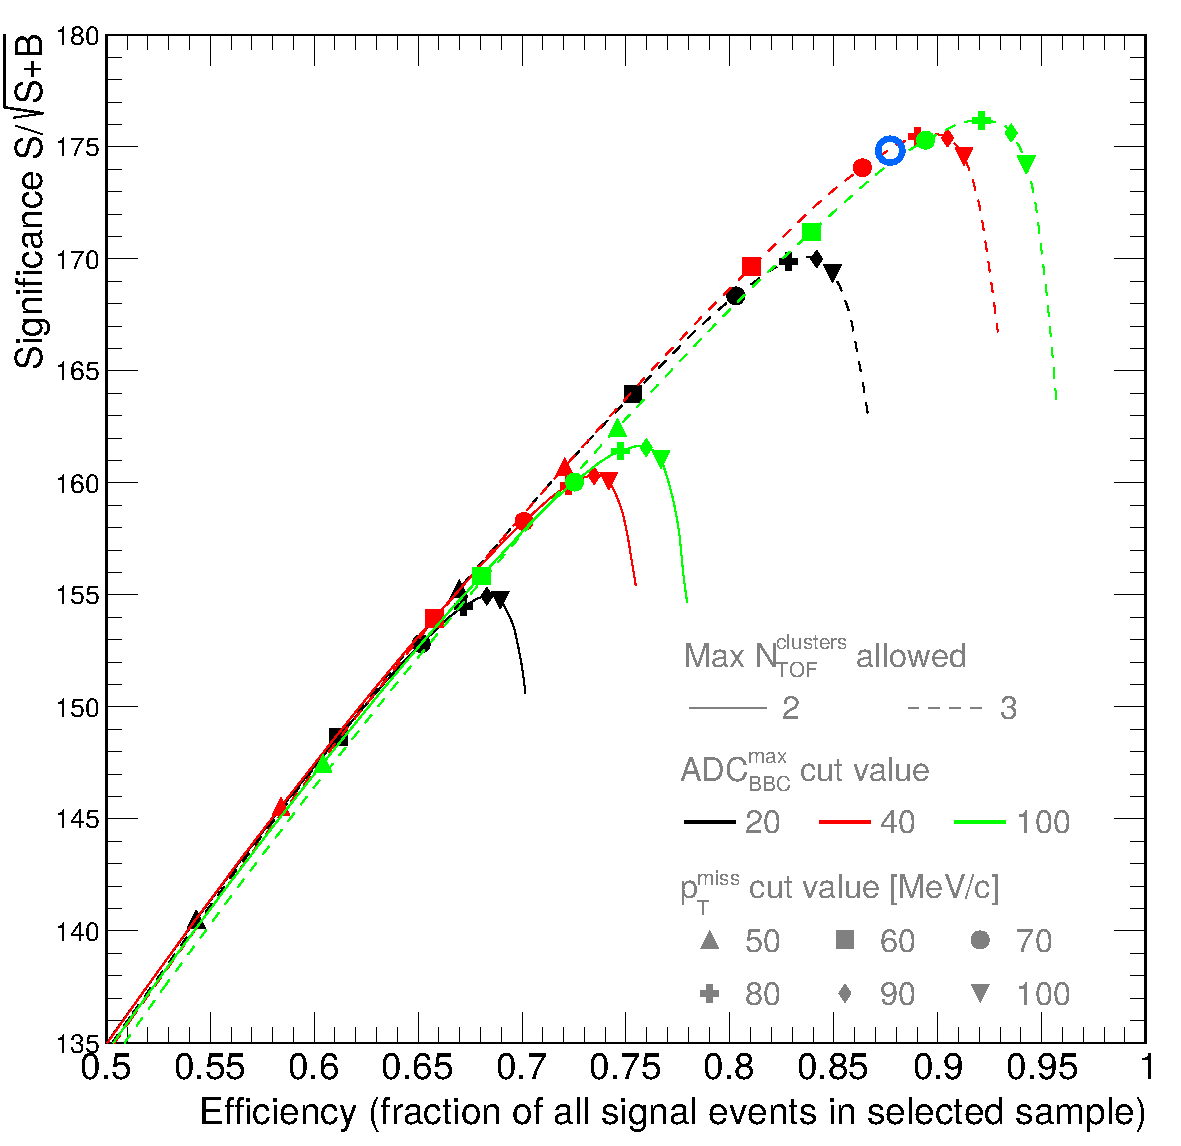
\includegraphics[width=\linewidth]{graphics/eventSelection/SignificanceVsEfficiency_pTmiss.pdf}}
  \end{subfigure}\\
  \begin{subfigure}[b]{\linewidth}\addtocounter{subfigure}{1}
                \subcaptionbox{\label{fig:EffVsBkgdFrac}}{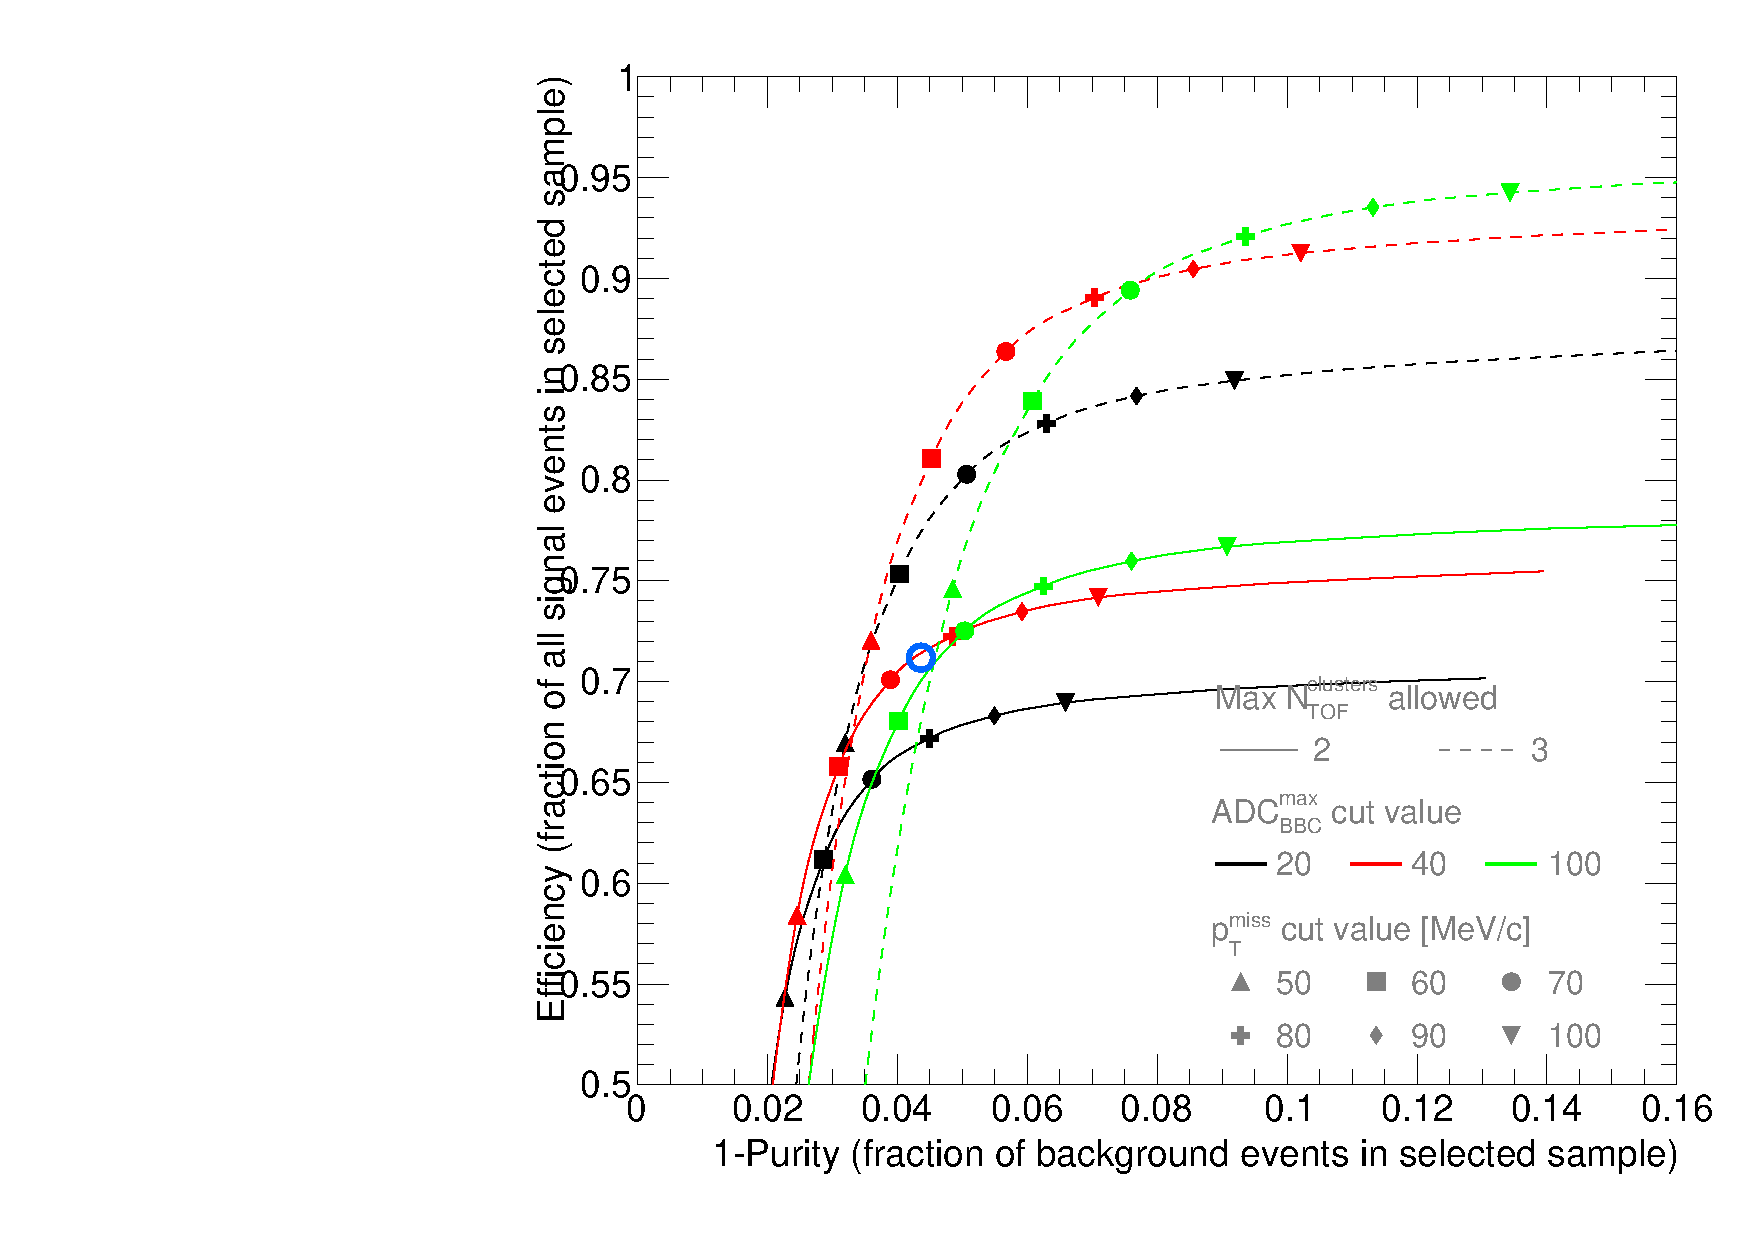
\includegraphics[width=\linewidth]{graphics/eventSelection/ROC_pTmiss.pdf}}
  \end{subfigure}
}%
\quad\quad%
\parbox{0.4725\textwidth}{
  \centering
  \begin{subfigure}[b]{\linewidth}\addtocounter{subfigure}{-2}
                \subcaptionbox{\label{fig:SignificanceVsBkgdFrac}}{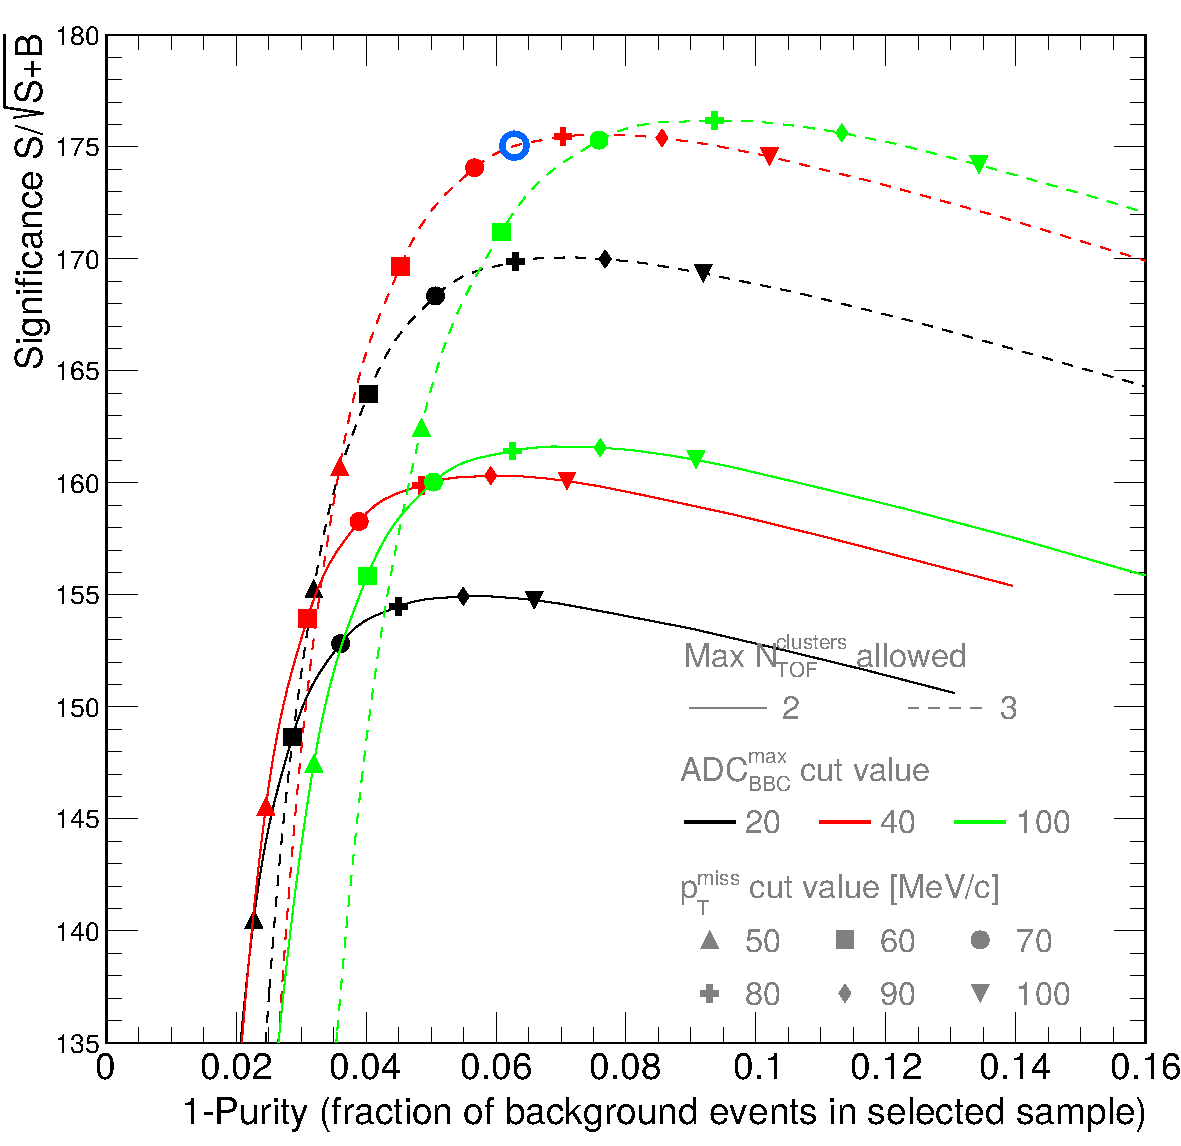
\includegraphics[width=\linewidth]{graphics/eventSelection/BkgdFractionVsEfficiency_pTmiss.pdf}}
  \end{subfigure}\\
  \begin{minipage}[t][1.042\linewidth][t]{\linewidth}\vspace{10pt}
    \caption[Relation between $\pi^{+}\pi^{-}$ significance, efficiency and purity vs. thresholds in cuts~\ref{enum:CutBbcLarge}, \ref{enum:CutTofClusters} and \ref{enum:CutMissingPt}]{Relation between $\pi^{+}\pi^{-}$ signal significance and efficiency (\subref{fig:SignificanceVsEff}), significance and purity (\subref{fig:SignificanceVsBkgdFrac}), and efficiency and purity (\subref{fig:EffVsBkgdFrac}) as a function of cut thresholds (the same for all channels) in BBC-large veto (\ref{enum:CutBbcLarge}), TOF cluster limit (\ref{enum:CutTofClusters}) and exclusivity cut (\ref{enum:CutMissingPt}). Lines show forementioned relations with changing $p_{T}^\text{miss}$ cut whose some specific values are indicated with different markers. Color denotes ADC threshold in BBC-large veto (black, red or green). Style of line (solid or dashed) denotes $N^{\text{TOF}}_{\text{clstrs}}$ limit. Working point considered optimal is marked with opened blue circle.}\label{fig:workingPoint}
  \end{minipage}
}%

\end{figure}\\
%--------------------------- 
In these equations $N_{\text{signal}}^{\text{cut}}$
